\section{Separable differential equations} \label{S:6.7.SolvingDE}

\begin{goals}
\item What is a separable differential equation?  
\item How can we find solutions to a separable differential equation?
\item Are some of the differential equations that arise in applications separable?
\item How can we use differential equations to describe and understand 
  phenomena in the world around us?
\end{goals} 

%---------------------------------------------
% SUBSECTION INTRODUCTION
%---------------------------------------------
\subsection*{Introduction}

Given the frequency with which differential equations arise in the world around us, we would like to have some techniques for finding explicit algebraic solutions of certain initial value problems.  In this section, we focus on a particular class of differential equations (called {\em separable}) and develop a method for finding algebraic formulas for solutions to these equations.

A {\em separable differential equation}\index{separable} is a differential equation whose algebraic structure permits the variables present to be separated in a particular way.  For instance, consider the equation
$$ \frac{dy}{dt} = ty. $$
We would like to separate the variables $t$ and $y$ so that all occurrences of $t$ appear on the right-hand side, and all occurrences of $y$ appears on the left and multiply $dy/dt$.  We may do this in the preceding differential equation by dividing both sides by $y$:
$$ \frac1y\frac{dy}{dt} = t. $$
Note particularly that when we attempt to separate the variables in a differential equation, we require that the left-hand side be a product in which the derivative $dy/dt$ is one term.  

Not every differential equation is separable.  For example, if we consider the equation
$$ \frac{dy}{dt} = t-y, $$
it may seem natural to separate it by writing
$$ y + \frac{dy}{dt} = t. $$
As we will see, this will not be helpful since the left-hand side is not a product of a function of $y$ with $\frac{dy}{dt}$.

\input{previews/6.7.PA1} %PREVIEW 

%--------------------------------------------------------------------------------
% SUBSECTION SEPERABLE DIFFERENTIAL EQUATIONS
%--------------------------------------------------------------------------------
\subsection*{Solving separable differential equations} \index{separable}

Before we discuss a general approach to solving a separable differential equation, it is instructive to consider an example.

%\begin{marginfigure} % MARGIN FIGURE
%\margingraphics{figures/6_4_DamEx.eps}
%\caption{A trapezoidal dam that is 25 feet tall, 60 feet wide at its base, 90 feet wide at its top, with the water line 5 feet down from the top of its face.} \label{F:6.4.DamEx}
%\end{marginfigure}

\begin{example} \label{eg:6.7.1} % EXAMPLE
Find all functions $y$ that are solutions to the differential equation 
$$\frac{dy}{dt}= \frac{t}{y^2}.$$

\solution We begin by separating the variables and writing
$$ y^2\frac{dy}{dt} = t. $$
Integrating both sides of the equation with respect to the independent variable $t$ shows that
$$ \int y^2\frac{dy}{dt}~dt = \int t~dt. $$
Next, we notice that the left-hand side allows us to change the variable of antidifferentiation from $t$ to $y$.  In particular, $dy = \frac{dy}{dt}~dt$, so we now have
$$ \int y^2 ~dy = \int t~dt. $$
This is why we required that the left-hand side be written as a product in which $dy/dt$ is one of the terms. This most recent equation says that two families of antiderivatives are equal to one another.  Therefore, when we find representative antiderivatives of both sides, we know they must differ by arbitrary constant $C$.  Antidifferentiating and including the integration constant $C$ on the right, we find that
$$ \frac{y^3}{3} = \frac{t^2}{2} + C. $$
    Again, note that it is not necessary to include an arbitrary constant on both sides 
    of the equation;  we know that $y^3/3$ and $t^2/2$ are in the same
    family of antiderivatives and must therefore differ by a single
    constant.

Finally, we may now solve the last equation above for $y$ as a function of $t$, which gives
    $$
    y(t) = \sqrt[3]{\frac 32 \thinspace t^2 + 3C}.
    $$
    Of course, the term $3C$ on the right-hand side represents
    $3$ times an unknown constant.  It is, therefore, still an unknown
    constant, which we will rewrite as $C$.  We thus conclude that the funtion
    $$
    y(t) = \sqrt[3]{\frac 32 \thinspace t^2 + C}
    $$
is a solution to the original differential equation for any value of $C$.

Notice that because this solution depends on the arbitrary constant $C$, we have found an infinite family of
solutions.  This makes sense because we expect to find a unique solution that corresponds to any given
 initial value.

For example, if we want to solve the initial value problem
$$
  \frac{dy}{dt} = \frac{t}{y^2}, \
  y(0) = 2,
$$
we know that the solution has the form $y(t) = \sqrt[3]{\frac32\thinspace
  t^2 + C}$ for some constant $C$.  We therefore must find the appropriate
value for $C$ that gives the initial value $y(0)=2$.  Hence,
$$
  2 = y(0)  \sqrt[3]{\frac 32 \thinspace 0^2 + C} = \sqrt[3]{C},
  $$
which shows that $C = 2^3 = 8$.  The solution to the initial value problem is then
$$
y(t) = \sqrt[3]{\frac32\thinspace t^2+8}.
$$
\end{example}  %EXAMPLE 

The strategy of Example~\ref{eg:6.7.1} may be applied to any differential equation of the form $\frac{dy}{dt} = g(y) \cdot h(t)$, and any differential equation of this form is said to be \emph{separable}.  We work to solve a separable differential equation by writing
$$\frac{1}{g(y)} \frac{dy}{dt} = h(t),$$ 
and then integrating both sides with respect to $t$.  After integrating, we strive to solve algebraically for $y$ in order to write $y$ as a function of $t$.

We consider one more example before doing further exploration in some activities.

%\begin{marginfigure} % MARGIN FIGURE
%\margingraphics{figures/6_4_DamEx.eps}
%\caption{A trapezoidal dam that is 25 feet tall, 60 feet wide at its base, 90 feet wide at its top, with the water line 5 feet down from the top of its face.} \label{F:6.4.DamEx}
%\end{marginfigure}

\begin{example} \label{eg:6.7.2} % EXAMPLE
Solve the differential equation
$$\frac{dy}{dt} =3y.$$

\solution Following the same strategy as in Example~\ref{eg:6.7.1}, we have
$$  \frac 1y \frac{dy}{dt} = 3. $$
Integrating both sides with respect to $t$,
$$  \int \frac 1y\frac{dy}{dt}~dt = \int 3~dt,$$
and thus 
$$ \int \frac 1y~dy =  \int 3~dt.$$
Antidifferentiating and including the integration constant, we find that
$$  \ln|y| = 3t + C.$$
Finally, we need to solve for $y$.  Here, one point deserves careful
attention.  By the definition of the natural logarithm function, it follows that
$$
|y| = e^{3t+C} = e^{3t}e^C.
$$
Since $C$ is an unknown constant, $e^C$ is as well, though we do know
that it is positive (because $e^x$ is positive for any $x$).
When we remove the absolute value in order to solve for $y$, however, this constant may be either positive or
negative.  We 
will denote this updated constant (that accounts for a possible $+$ or $-$) by $C$ to obtain
$$
y(t) = Ce^{3t}.
$$

There is one more slightly technical point to make.  Notice that $y=0$
is an equilibrium solution to this differential equation.  In solving
the equation above, we begin by dividing both sides by $y$, which
is not allowed if $y=0$.  To be perfectly careful, therefore, we will typically
consider the equilibrium solutions separably.  In this case, notice that the final
form of our solution captures the equilibrium solution by allowing
$C=0$. 
\end{example}  %EXAMPLE 

\input{activities/6.7.Act1}  %ACTIVITY   

\input{activities/6.7.Act2} %ACTIVITY

\begin{activity} \label{A:7.4.3}  Solve each of the following differential equations or initial value problems.
\ba
	\item $\ds \frac{dy}{dt} - (2-t) y = 2-t$
	\item $\ds \frac{1}{t}\frac{dy}{dt} = e^{t^2-2y}$
	\item $y' = 2y+2$, \ \ $y(0)=2$
	\item $y' = 2y^2$, \ \ $y(-1) = 2$
	\item $\ds \frac{dy}{dt} = \frac{-2ty}{t^2 + 1}$, \ \  $y(0) = 4$
\ea
\end{activity}
\begin{smallhint}
\ba
	\item Small hints for each of the prompts above.
\ea
\end{smallhint}
\begin{bighint}
\ba
	\item Big hints for each of the prompts above.
\ea
\end{bighint}
\begin{activitySolution}
\ba
	\item Solutions for each of the prompts above.
\ea
\end{activitySolution}
\aftera %ACTIVITY


%--------------------------------------------------------------------------------
% SUBSECTION SEPERABLE DIFFERENTIAL EQUATIONS
%--------------------------------------------------------------------------------
\subsection*{Developing a differential equation}

In our work to date, we have seen several ways that
differential equations arise in the natural world, from the growth of
a population to the temperature of a cup of coffee.  Now,
we will look more closely at how differential equations give us a
natural way to describe various phenoma.  As we'll see, the key is to
focus on understanding the different factors that cause a quantity to
change.

\input{activities/6.7.Act4} % ACTIVITY

Activity~\ref{A:6.7.4} demonstrates the kind of thinking we will be
doing.  In each of the two examples we considered, there is a
quantity, such as the amount of money in the bank account or the
amount of salt in the tank, that is changing due to several factors.
The governing differential equation results from the total rate of change being the difference between the rate of
increase and the rate of decrease.

\begin{marginfigure}[8cm] % MARGIN FIGURE
\margingraphics{figures/7_5_lake_michigan.eps}
\caption{Plot of $\frac{dP}{dt}$ vs. $P$. } \label{F:6.7.Ex3-1}
\end{marginfigure}

\begin{example} \label{eg:6.7.3} % EXAMPLE
In the Great Lakes region, rivers flowing into the lakes carry a great
deal of pollution in the form of small pieces of plastic averaging $1$
millimeter in diameter.  In order to understand how the amount of
plastic in Lake Michigan is changing, construct a model for how this type pollution has built up in the lake.


\solution First, some basic facts about Lake Michigan.
\begin{itemize}
  \item The volume of the lake is
    $5\cdot10^{12}$ cubic meters.
  \item Water flows into the lake at a rate of
    $5\cdot10^{10}$ cubic meters per year.  It flows out of the lake
    at the same rate.
  \item Each cubic meter flowing
    into the lake contains roughly $3\cdot10^{-8}$ cubic meters of
    plastic pollution.
\end{itemize}

Let's denote the amount of pollution in the lake by $P(t)$, where $P$
is measured in cubic meters of plastic and $t$ in years.  Our goal
is to describe the rate of change of this function;  in other
words, we want to develop a differential equation describing $P(t)$.

First, we will measure how $P(t)$ increases due to pollution flowing
into the lake.  We know that $5\cdot10^{10}$ cubic meters of water
enters the lake every year and each cubic meter of water contains
$3\cdot10^{-8}$ cubic meters of pollution.  Therefore, pollution
enters the lake at the rate of
$$ \left(5\cdot 10^{10} \frac{m^3 \mbox{\ water}}{\mbox{year}}\right) \cdot \left(3\cdot10^{-8} \frac{m^3 \mbox{\ plastic}}{m^3 \mbox{\ water}} \right) = 1.5\cdot 10^3$$
cubic meters of plastic per year.

Second, we will measure how $P(t)$ decreases due to pollution flowing
out of the lake.  If the total amount of pollution is $P$ cubic
meters and the volume of Lake Michigan is $5\cdot 10^{12}$ cubic
meters, then the concentration of plastic pollution in Lake Michigan is
$$
\frac{P}{5\cdot10^{12}} \quad \hbox{cubic meters of plastic per cubic meter of water}.
$$
Since $5\cdot10^{10}$ cubic meters of water flow out each year,and we assume that each cubic meter of water that flows out carries with it the plastic pollution it contains, then
the plastic pollution leaves the lake at the rate of
$$ \left(\frac{P}{5\cdot10^{12}} \frac{m^3 \mbox{\ plastic}}{m^3 \mbox{\ water}} \right) \cdot \left(5\cdot10^{10} \frac{m^3 \mbox{\ water}}{\mbox{year}} \right)=\frac{P}{100} $$
cubic meters of plastic per year.

The total rate of change of $P$ is thus the difference between the rate at which
pollution enters the lake minus the rate at which pollution leaves the
lake;  that is,
\begin{eqnarray*}
\frac{dP}{dt} & = &1.5\cdot10^{3}-\frac{P}{100} \\
                   & = & \frac{1}{100}(1.5\cdot10^{5} - P).
\end{eqnarray*}

We have now found a differential equation that describes the rate
at which the amount of pollution is changing.  To better understand the
behavior of $P(t)$, we now apply some
of the techniques we have recently developed.

Since this is an autonomous differential equation, we can sketch
$dP/dt$ as a function of $P$ and then construct a slope field, as shown in Figure~\ref{F:6.7.Ex3-1} and Figure \ref{F:6.7.Ex3-2}.

These plots both show that $P=1.5\cdot10^5$ is a stable equilibrium.  Therefore,
we should expect that the amount of pollution in Lake Michigan will
stabilize near $1.5\cdot10^5$ cubic meters of pollution.

Next, assuming that there is initially no pollution in the lake, we will
solve the initial value problem
$$
\frac{dP}{dt} = \frac{1}{100}(1.5\cdot10^{5} - P), \ P(0) = 0.
$$
Separating variables, we find that
$$
\frac1{1.5\cdot10^5-P} \frac{dP}{dt} = \frac1{100}.
$$
Integrating with respect to $t$, we have 
$$  \int \frac1{1.5\cdot10^5-P} \frac{dP}{dt}~dt = \int \frac1{100}~dt,$$
and thus changing variables on the left and antidifferentiating on both sides, we find that
\begin{eqnarray*}
  \int \frac{dP}{1.5\cdot10^5-P} &=& \int \frac1{100}~dt \\
  -\ln|1.5\cdot10^5 - P| & = & \frac1{100}t + C
\end{eqnarray*}
Finally, multiplying both sides by $-1$ and using the definition of the logarithm, we find that
\begin{equation} \label{E:7.5.Ex1C}  1.5\cdot10^5 - P = C e^{-t/100}.
\end{equation}
This is a good time to determine the constant $C$.  Since $P =
0$ when $t=0$, we have
$$
1.5\cdot 10^5 - 0 = Ce^0 = C.
$$
In other words, $C=1.5\cdot10^5$. 

Using this value of $C$ in Equation~(\ref{E:7.5.Ex1C}) and solving for $P$, we arrive at the solution
$$ P(t) = 1.5\cdot10^5(1-e^{-t/100}).$$
Superimposing the graph of $P$ on the slope field we saw in Figure \ref{F:6.7.Ex3-1} and Figure \ref{F:6.7.Ex3-2}, we see, as shown in Figure~\ref{F:6.7.Ex3-3}.

We see that, as expected, the amount of plastic pollution stabilizes around
$1.5\cdot10^5$ cubic meters.
\end{example}

\begin{marginfigure}[-16cm] % MARGIN FIGURE
\margingraphics{figures/7_5_slope_field.eps}
\caption{The slope field for the differential equation $\frac{dP}{dt} = \frac{1}{100}(1.5\cdot10^{5} - P)$.} \label{F:6.7.Ex3-2}
\end{marginfigure}

\begin{marginfigure}[-4cm] % MARGIN FIGURE
\margingraphics{figures/7_5_solution.eps}
\caption{The solution $P(t)$ and the slope field for the differential equation $\frac{dP}{dt} = \frac{1}{100}(1.5\cdot10^{5} - P)$.} \label{F:6.7.Ex3-3}
\end{marginfigure}  % EXAMPLE ***Don't forget the figures!!***

There are many important lessons to learn from Example~\ref{eg:6.7.3}.  Foremost is how we can develop a differential equation by thinking about the ``total rate = rate in - rate out'' model.  In addition, we note how we can bring together all of our available understanding (plotting $\frac{dP}{dt}$ vs. $P$, creating a slope field, solving the differential equation) to see how the differential equation describes the behavior of a changing quantity.

Of course, we can also explore what happens when certain aspects of the problem change.  For instance, let's suppose we are at a time when the plastic pollution entering Lake Michigan has
stabilized at $1.5\cdot10^5$ cubic meters, and that new legislation is
passed to prevent this type of pollution entering the lake.  So, there is no longer any inflow of plastic pollution to the lake.  How does the amount of plastic pollution in Lake Michigan now change?  For example, how long does it take for the amount of plastic pollution in the lake to halve?

Restarting the problem at time $t=0$, we now have the modified initial value problem
$$
\frac{dP}{dt} = -\frac{1}{100}P, \ P(0) = 1.5\cdot10^5.
$$
It is a straightforward and familiar exercise to find that the solution to this equation is $P(t) = 1.5\cdot10^5
e^{-t/100}$.  The time that it takes for half of the pollution to flow
out of the lake is given by $T$ where $P(T) = 0.75\cdot10^5$.  Thus, we must solve the equation
$$0.75\cdot10^5 = 1.5\cdot10^5e^{-T/100},$$
or
$$ \frac12 = e^{-T/100}.$$
It follows that 
$$T = -100\thinspace\ln\left(\frac12\right) \approx 69.3 \quad\hbox{years.}$$

In the activities that follow, we explore some other natural settings in which differential equation model changing quantities.

\input{activities/6.7.finance} %ACTIVITY

\input{activities/6.7.iv.drug} %ACTIVITY


%--------------------------------------------------------------------------------
% SUBSECTION POPULATION GROWTH
%--------------------------------------------------------------------------------
\subsection*{Population Growth}

We will now begin studying the earth's population.  To get started, some data for the earth's population in recent years that we will use in our investigations is given in Table~\ref{T:earthpop}.

\begin{margintable}[6cm]

\begin{center}
\scalebox{1.25}{
  \begin{tabular}{|c|c|}
    \hline
    Year & Population \\
    \hline
    $1998$ & $5.932$ \\
    $1999$ & $6.008$ \\
    $2000$ & $6.084$ \\
    $2001$ & $6.159$ \\
    $2002$ & $6.234$ \\
    $2005$ & $6.456$ \\
    $2006$ & $6.531$ \\
    $2007$ & $6.606$ \\
    $2008$ & $6.681$ \\
    $2009$ & $6.756$ \\
    $2010$ & $6.831$ \\
    \hline
  \end{tabular}
} % end scalebox
\end{center}

\caption{The earth's recent population (in billions).}
\label{T:earthpop}
\end{margintable}

\input{activities/6.7.exponential} %ACTIVITY

Our work in Activity~\ref{A:7.6.1} shows that that the exponential model is fairly accurate for years 
relatively close to $2000$.  However, if we go too far into the
future, the model predicts increasingly large rates of change, which
causes the population to grow arbitrarily large.  This does not make
much sense since it is unrealistic to expect that the earth would be able to support
such a large population.  

The constant $k$ in the differential equation has an important
interpretation.  Let's rewrite the differential equation $\frac{dP}{dt} = kP$ by solving for $k$, so that we have
$$k = \frac{dP/dt}{P}.$$
Viewed in this light, $k$ is the ratio of the rate of change to the
population;  in other words, it is the contribution to the rate of change 
from a single person.  We call this the {\em per capita
  growth rate}\index{per capita growth rate}.

In the exponential model we introduced in Activity~\ref{A:7.6.1}, the per capita growth rate is
constant.  In particular, we are assuming that when the population is
large, the per capita growth rate is the same as when the population
is small.  It is natural to think that the per capita growth rate should
decrease when the population becomes large, since there will not be
enough resources to support so many people.  In other words, we expect that a more realistic model would hold if we assume
that the per capita growth rate depends on the population $P$.

In the previous activity, we computed the per capita growth rate in a
single year by computing $k$, the quotient of $\frac{dP}{dt}$ and $P$ (which we did for $t = 0$).  If we return data and compute the per capita
growth rate over a range of years, we generate the data shown in Figure~\ref{F:6.7.census}-(a), which shows how the per capita growth rate is a function of the population, $P$.  

From the data, we see that the per capita growth rate appears to decrease as
the population increases.  In fact, the points seem to lie very close
to a line, which is shown at two different scales in Figure \ref{F:6.7.census}-(b) and Figure \ref{F:6.7.census}-(c).

\begin{marginfigure}[-6cm] % MARGIN FIGURE
\begin{center}
\subfloat[]{\includegraphics[scale=.75]{figures/7_6_census.eps}}

\subfloat[]{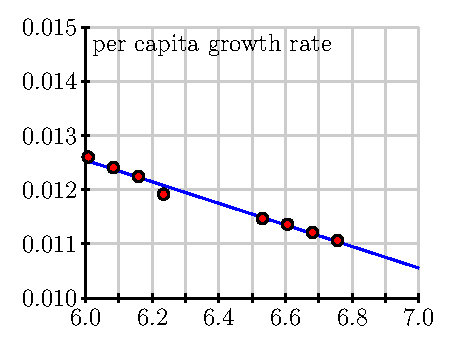
\includegraphics[scale=.75]{figures/7_6_census_1.eps}}

\subfloat[]{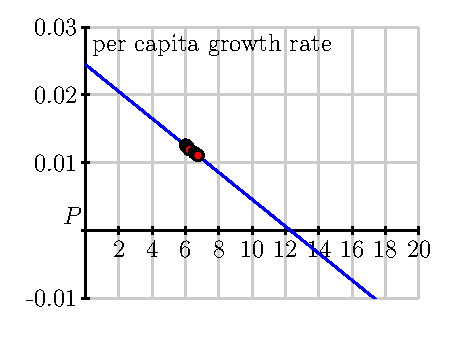
\includegraphics[scale=.75]{figures/7_6_census_2.eps}}
\end{center}
\caption{The data and approximations of the per capita growth as a function of population, $P$.}
\label{F:6.7.census}
\end{marginfigure}

Looking at this line carefully, we can find its equation to be
$$
\frac{dP/dt}{P} = 0.025 - 0.002P.
$$
If we multiply both sides by $P$, we arrive at the differential
equation
$$
\frac{dP}{dt} = P(0.025 - 0.002P).
$$
Graphing the dependence of $dP/dt$ on the population $P$, we see that this differential equation demonstrates a quadratic relationship between $\frac{dP}{dt}$ and $P$, as shown in Figure~\ref{F:6.7.logistic}.

The equation $\frac{dP}{dt} = P(0.025 - 0.002P)$ is an example of the {\em logistic equation}, 
and is the second model for population growth that we will consider.  We
have reason to believe that it will be more realistic since the per
capita growth rate is a decreasing function of the population.

Indeed, the graph in Figure~\ref{F:6.7.logistic} shows that there are two equilibrium
solutions, $P=0$, which is unstable, and $P=12.5$, which is a stable
equilibrium.  The graph shows that any solution with $P(0) >0$ will
eventually stabilize around $12.5$.  In other words, our model predicts
the the world's population will eventually stabilize around $12.5$
billion.

\begin{marginfigure}
  \margingraphics{figures/7_6_logistic_de.eps}
  \caption{A plot of $\frac{dP}{dt}$ vs.~$P$ for the differential equation $\frac{dP}{dt} = P(0.025 - 0.002P)$.}
  \label{F:6.7.logistic}
\end{marginfigure}

A prediction for the long-term behavior of the population is a
valuable conclusion to draw from our differential equation.  We would,
however, like to answer some quantitative questions.  For instance,
how long will it take to reach a population of $10$ billion?  To determine this,
we need to find an explicit solution of the equation.  

%--------------------------------------------------------------------------------
% SUBSECTION LOGISTIC DIFFERENTIAL EQUATION
%--------------------------------------------------------------------------------
\subsection*{Solving the logistic differential equation} \index{logistic}

Since we would like to apply the logistic model in more general situations, we state the logistic equation\index{logistic equation} in its more general form,
\begin{equation} \label{E:6.7.logistic}
\frac{dP}{dt} = kP(N-P).
\end{equation}
The equilibrium solutions here are when $P=0$ and $1-\frac PN = 0$,
which shows that $P=N$.  The equilibrium at $P=N$ is called the {\em
  carrying capacity}\index{carrying capacity} of the population for it represents the stable
population that can be sustained by the environment.

We now solve the logistic equation~(\ref{E:6.7.logistic}).  The equation is separable, so we separate the variables
$$
\frac{1}{P(N-P)}\frac{dP}{dt} = k,
$$
and integrate to find that
$$
\int \frac{1}{P(N-P)}~dP = \int k~dt.
$$

To find the antiderivative on the left, we use the partial fraction decomposition
$$
\frac{1}{P(N-P)} = \frac 1N\left[\frac 1P + \frac 1{N-P}\right].
$$
Now we are ready to integrate, with 
$$
\int \frac 1N\left[\frac 1P + \frac 1{N-P}\right] ~dP  =  \int k~dt. 
$$
On the left, observe that $N$ is constant, so we can remove the factor of $\frac{1}{N}$ and antidifferentiate to find that
$$
\frac 1N (\ln|P| - \ln|N-P|)  =  kt + C.
$$
Multiplying both sides of this last equation by $N$ and using an important rule of logarithms, we next find that
$$\ln\left|\frac{P}{N-P}\right| = kNt + C.$$
From the definition of the logarithm, replacing $e^C$ with $C$, and letting $C$ absorb the absolute value signs, we now know that 
$$\frac{P}{N-P} =  Ce^{kNt}.$$
At this point, all that remains is to determine $C$ and solve algebraically for $P$.

If the initial population is $P(0) = P_0$, then it follows that $C = \frac{P_0}{N-P_0}$, so
$$\frac{P}{N-P} = \frac{P_0}{N-P_0}e^{kNt}.$$
We will solve this most recent equation for $P$ by multiplying both sides by
$(N-P)(N-P_0)$ to obtain 
\begin{eqnarray*}
P(N-P_0) &=& P_0(N-P)e^{kNt}  \\
	 &=& P_0Ne^{kNt} - P_0Pe^{kNt}. 
\end{eqnarray*}	 
Swapping the left and right sides, expanding, and factoring, it follows that
\begin{eqnarray*}
P_0Ne^{kNt} & = & P(N-P_0) + P_0 Pe^{kNt}  \\
	& = & P(N-P_0 + P_0e^{kNt}). 
\end{eqnarray*}
Dividing to solve for $P$, we see that
$$P = \frac{P_0Ne^{kNt}}{N-P_0 + P_0e^{kNt}}.$$
Finally, we choose to multiply the numerator and denominator by $\frac{1}{P_0}e^{-kNt}$
to obtain
$$
P(t) = \frac{N}{\left(\frac{N-P_0}{P_0}\right) e^{-kNt} + 1}.
$$

While that was a lot of algebra, notice the result:  we have
found an explicit solution to the initial value problem
$$
  \frac{dP}{dt} = kP(N-P), \ P(0) = P_0,
$$
and that solution\index{logistic equation!solution} is 
\begin{equation}\label{E:7.6.logistic_solution}
P(t) = \frac{N}{\left(\frac{N-P_0}{P_0}\right) e^{-kNt} + 1}.
\end{equation}

For the logistic equation describing the earth's population that we worked with earlier in this section, we have
$$k=0.002, \quad N= 12.5, \quad \hbox{and} \quad P_0 = 6.084.$$
This gives the solution
$$
P(t) = \frac{12.5}{1.0546e^{-0.025t} + 1},
$$
whose graph is shown in Figure~\ref{F:6.7.logistic_sol}
\begin{marginfigure} 
 \margingraphics{figures/7_6_logistic_sol.eps}
\caption{The solution to the logistic equation modeling the earth's population.} \label{F:6.7.logistic_sol}
\end{marginfigure}

Notice that the graph shows the population leveling off at $12.5$ billion, as
we expected, and that the population will be around $10$ billion in the
year $2050$.  These results, which we have found using a relatively simple
mathematical model, agree fairly well with predictions made using a
much more sophisticated model developed by the United Nations.

The logistic equation is useful in other situations, too, as it is good for modeling any situation in which limited growth is possible.  For instance, it could model the spread of a flu virus through a population contained on a cruise ship, the rate at which a rumor spreads within a small town, or the behavior of an animal population on an island.  Again, it is important to realize that through our work in this section, we have completely solved the logistic equation, regardless of the values of the constants $N$, $k$, and $P_0$.  Anytime we encounter a logistic equation, we can apply the formula we found in Equation~(\ref{E:7.6.logistic_solution}).

\input{activities/6.7.logistic} %ACTIVITY


%---------------------
% SUMMARY
%---------------------
\begin{summary}
\item A separable differential equation is one that may be rewritten
  with all occurrences of the dependent variable multiplying the
  derivative and all occurrences of the independent variable on the
  other side of the equation.
\item We may find the solutions to certain separable differential equations
  by separating variables, integrating with respect to $t$, and ultimately solving the resulting algebraic equation for $y$.
 
\item This technique allows us to solve many important differential
  equations that arise in the world around us.  For instance, questions of
  growth and decay and Newton's Law of Cooling give rise to separable
  differential equations.  

\item If we assume that the rate of growth of a population is
  proportional to the population, we are led to a model in which the
  population grows without bound and at a  rate that grows without bound. 
\item By assuming that the per capita growth rate decreases as the
  population grows, we are led to the logistic model of population
  growth, which predicts that the population will eventually
  stabilize at the carrying capacity.    
\end{summary}

\clearpage

%--------------
% EXERCISES
%--------------
\input{exercises/6-7.Seperable(Ex)} 

\cleardoublepage